\chapter{Text Mining}\label{Text Mining}

Nu men een algemeen begrip heeft van wat machine learning juist is en welke algemene technieken het omvat, kan men overgaan naar text mining en zijn geschikte technieken. In dit hoofdstuk gaat men bespreken welke technieken men kan gebruken voor text mining en wat deze juist inhouden. Als laatste gaat men de theorie toepassen op een voorbeeld en gaat men de resultaten van dit experiment bespreken. 
\newline
%
Text mining of text data mining is een techniek waarbij men aan tekstanalyse doet om zo trends en patronen te kunnn vaststelllen. Neem opnieuw als voorbeeld onze artikels. Met text mining wil men de artikels zodanig analyseren zodanig dat men kan uitmaken welk artikel positief en welk negatief is.
Een probleem dat zich onmiddelijk bij text mining voordoet is het ontbreken van een  \'e\'en-op-\'en relatie van woorden en een concept. Woorden verwijzen zelfden eenduidig naar één concept. Zo het voorkomen van het woord "bank" in een tekst zowel verwijzen naar de finaciele instelling als naar een doodgewone zitbank in het park. Dergelijke dubbele betekenis van woorden maakt het moeilijk om de woorden, met als gevolg ook de tekst, te mappen op een bepaald concept.
%
Verder heeft men ook woorden in een tekst die weinig bijdragen tot de bepaling van het concept van de tekst bijvoorbeeld: ik,en,want...
Deze woorden kan men uit de tekst filteren door een database aan te leggen met woorden die moeten men moet negeren. Deze techniek en nog soortgelijke alternatieven vereisen dat er al een voorverwerking plaatsvindt voordat men de dataset echt gaat analyseren op patronenen trends. Algemeen kan men zeggen als men de resultaten van de text mining wil optimaliseren, men aan \textbf{\textit{document pre-processing}} moet doen.

\section{Document Pre-processing }\label{Document Pre-processing}

Document pre-processing is een optionele, maar zeker nuttig stap in het text mining proces. Document pre-processing bestaat eruit om je dataset al eens te verwerken, zodanig je extra informatie hebt, die je kan gebruiken bij de eigelijke analyse van de dataset. Zo kan je bijvoorbeeld alle stopwoorden verwijderen uit de dataset. Wanneer men dan op deze gewijzigde dataset een analyze uitvoert, geeft men indirect de informatie mee dat stopwoorden er niet toe doen. Uiteraard is het verwijderen van stopwoorden \'e\'en van de technieken.  Er bestaan nog andere technieken die nuttig zijn als voorverwerking van een dataset. Zo kan men tekst en stucturen afleiden. Bijvoorbeeld het omzetten van Microsoft Word of Latex documenten naar XML maakt het parsen en analyseren van de documenten voor het algoritme veel gemakkelijker.Verder kan men ook \textbf{\textit{stemming}} toepassen. Stemming is een techniek waarbij men tracht om de stam van het woord te achterhalen. Bijvoorbeeld uit het woord \textit{katachtig} kan men het woord \textit{kat} afleiden. De techniek kan gebaseerd zijn op een woordenboek bijvoorbeeld \textit{Mmorph} is zo'n stemming woordenboek ontwikkeld door de Universiteit van Gen\`eve. Verder kan men de stemming ook baseren op een set van regels, bepaald door taalkundige. Het onderstaande voorbeeld illustreert een set van stemming regels voor het Frans:

%Voorbeeld van stemming regels   
\newline
\begin{center}
  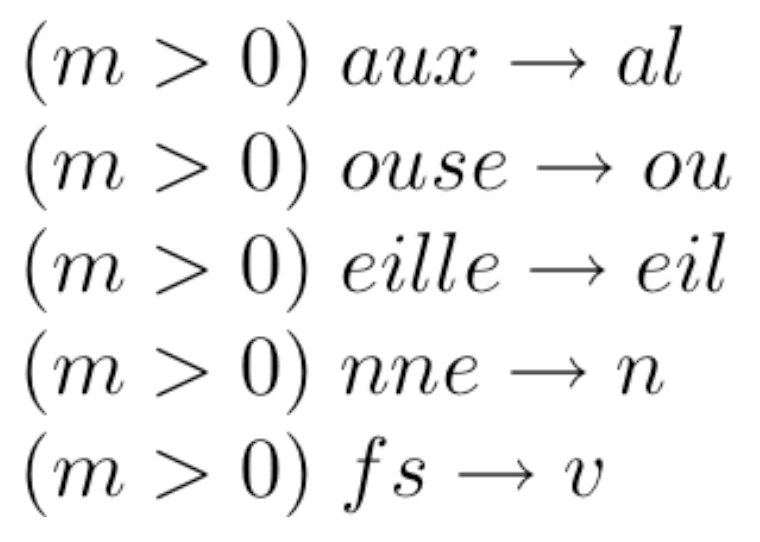
\includegraphics[width=5cm]{stemming_regels_frans}
  \captionof{figure}{Voorbeeld van stemming regels in het Frans}
\end{center}
%%
Tenslotte is \textbf{\textit{named entity recognition}} (NER) ook een techniek die men kan gebruiken bij document pre-processing. Hierbij gaat men entiteiten proberen detecteren in de tekst en deze labelen. Neem bijvoorbeeld de zin \textit{Yannick heeft zich ingeschreven de richting Computerwetenschappen aan de Vrije Universiteit Brussel in 2012}. Men kan met NER de entiteiten eruit halen, labelen en volgend resultaat verkrijgen: \textit{$\text{[Yannick]}_{persoon}$ heeft zich ingeschreven de richting Computerwetenschappen aan de $\text{[Vrije Universiteit Brussel]}_{organisatie}$ in $\text{[2012]}_{tijdsaanduiding}$}
\newline
Algemeen ziet men dat al deze technieken samen worden gecombineerd, wat alleen maar de uiteindelijke resultaten ten goede komt. Hoe deze gecombineerd kunnen wordt in het onderstaande voorbeeld ge\"illustreerd. 
\newline
\begin{center}
  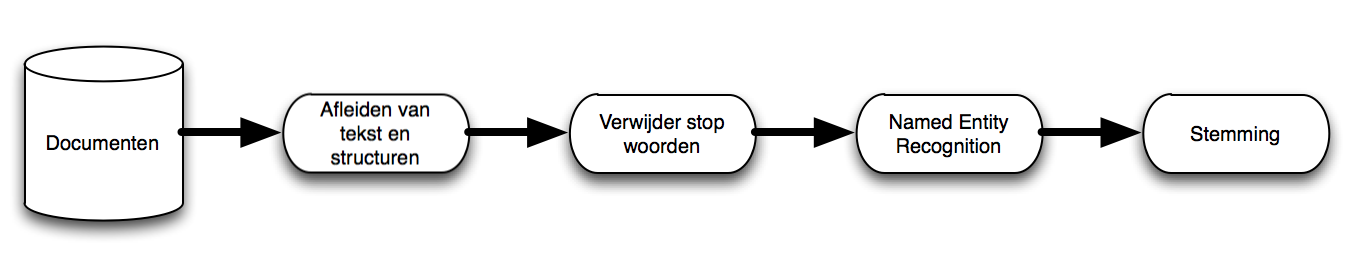
\includegraphics[width=10cm]{document_preprocessing}
  \captionof{figure}{Combinatie van technieken bij document pre-processing}
\end{center}

\section{Methoden}\label{Methoden}
Na de document pre-proccesing kan men beginnen aan de eigelijk analyse van de dataset. Voor de text mining kan men 2 methodes gebruiken: de vector space methode en  probablistic methode.
\subsection{Vector Space Methode}\label{Vector Space Methode}
De vector space methode is een methode waarbij men in principe een document als een vector voorsteld waarbij ieder elemenent overeenkomt met een woord en zijn frequentie in het document. Als men concreet een document voorsteld kan men zeggen dat document $j$ voorgesteld wordt door $\textbf{d}_{j}$ met $f_{ij}$ de frequentie van het woord $w_{i}$. Het aantal woorden stelt men voor door $n_{w}$, wat eveneens de dimensie is van de vector.
Het document kan dus als volgt worden voorgesteld:

\[ d_{j}  = \begin{bmatrix}
    f_{1j} \\
    f_{2j} \\
    \vdots \\
    f_{n_{w}j} \\
\end{bmatrix}  
\]
%
Een belangrijk inzicht bij het vector space methode is dat een document voorgesteld wordt als een groep van woorden. Er wordt geen rekening gehouden met de volgorde waarin de woorden in het document voorkomen. Vaak ziet men ook dat de vector vaak ijl is en vanwege de grote hoeveelheid aan woorden in een document heel groot. Als men nu niet \'e\'en doucument maar meerdere documenten neemt en men zegt dat het aantal documenten gelijk is aan $n_{d}$. Dit resulteert in een matrix waarbij iedere kolom een document voorsteld.
\[
D =
 \stackrel{\mbox{Documenten}}{%
    \begin{bmatrix}
    f_{11} & f_{12} & \cdots & f_{1n_{d}} \\
    f_{21} & f_{22} & \cdots & f_{2n_{d}} \\
    \vdots & \vdots & \ddots & \vdots \\
    f_{n_{w}j} & f_{n_{w}2} & \cdots & f_{n_{w}n_{d}}
    \end{bmatrix}
    }
    & Woorden \]
%
Deze matrix wordt ook een \textbf{\textit{terms-documents matrix (TDM)}} genoemd. Wanneer men spreekt van een  \textbf{\textit{documents-terms matrix (DTM)}}, spreekt men een getransponeerde terms-documents matrix. Een rij van een DTM stelt dan een document voor.
%
Maar hoe brengt deze voorstelling ons dichter bij het vinden van verbanden tussen de documenten? Wel men kan aan de hand van de euclidische afstand bepalen of documenten gelijkaardig zijn of niet. Stel men heeft twee documenten met een kleine euclidische afstand. Dit wil eigelijk zeggen dat de vectorvoorstelling van de documenten geljkaardig is. Wat wil zeggen dat de woordfrequenties ongeveer overeen komen en dus bijvoorbeeld de documenten over hetzelfde onderwerp gaan of eenzelfde mening uitdrukken.
%
In de praktijk is gebleken dat documenten vergelijken op basis van woordfrequentie nog niet de gewenste resultaten opleverd. Vaak is het nog altijd moeilijk om verschillend groepen tussen de documenten te onderscheiden. Daarom kan men nog extra verfijningen toepassen aan de hand van \textbf{\textit{term weighting}} en \textbf{\textit{Latent Semantic Models (LSM)}}.


\subsubsection{Term weigthing}\label{Term weighting}

Als men even stil staat bij onze TDM met woordfrequenties, kan men zeggen dat niet elk woord evenveel doorweegt. Een woord dat in alle documenten voorkomt biedt geen of minder waardevolle informatie, dan een woord dat zelden voorkomt. En hierop baseerd term weighthing zich. Het gaat een wegingsfactor introduceren. Ieder woord krijgt een gewicht toegewezen, dat weergeeft hoe belangrijk het woord is. Neem als voorbeeld een hoop recensies van de film "Pulp Fiction" en de woorden "Pulp" en "excellent". "Pulp" is een woord dat voorkomt in de titel van de film en komt ongetwijfeld in elke recensie voor. "Excellent" daarin tegen is een woord dat enkel maar voorkomt wanneer de recensist de film fantastisch vond, het zal niet in elk document voorkomen en is waardevolle informatie. Term weighting zal dus bij dit voorbeeld "excellent" een grotere gewicht toewijzen dan "Pulp". 
%
De quantiteit van dit gewicht wordt vaak de \textbf{inverse document frequency  (idf)} genoemd en wordt bepaald aan de hand van volgende formule:

\[w_{i}: idf_{i} = -log_{2}[P(w_{i})] \] \text{met $P(w_{i})$ dat priori probability dat word $w_{i}$ voorkomt in het document} 
%
In woorden geeft de inverse document frequency het algemeen belang van het woord $w_{i}$ weer. Men kan dit benaderen door het logarithme te nemen van het aantal documenten waar $w_{i}$ in voorkomt en het totaal aantal documenten.
Een andere nuttige quantiteit is de  \textbf{term frequency} $tf_{ij}$. Deze geeft het belang weer van het woord $w_{i}$ binnen in het document $d_{j}$  en wordt als volgt genoteerd:
\[ tf_{ij} = \frac{f_{ij}}{ \sum_{i=1}^{n_{w}}f_{ij}} \]
%
Met deze twee quantiteiten kan men een nieuwe begrip introduceren: de textbf{tf-idf score}. Wat overeenkomt met het product van tf en idf.
 
\[ \text{tf-idf score} = tf . idf_{ij} = idf_{i} . tf_{ij} \]
%
De tf-idf matrix bekomt men dan door alle woordfrequenties van het terms-document matrix te vervangen door de tf-idf score.
Deze matrix wordt bijvoorbeeld vaak gebruikt om de gelijkenissen tussen twee documenten te bepalen op basis van cosinusgeljkenis


\subsubsection{Latent Semantic Models}\label{Latent Semantic Models}

Als tweede verfijninig van het vector space model, heeft men latent sementic models (LSM). Met LSM probeert men een notie te krijgen van de semantische informatie en maar bepaald het semantisch verband tussen woorden. Bijvoorbeeld als men zoekt naar documenten met het woord "economie", men ook documenten met "financi\"en" zou terugkrijgen. Voor LSM zijn twee woorden semantisch gerelateerd als ze gebruikt worden in dezelfde context. Met het concrete voorbeeld kunnen we zeggen dat er een semantisch verband is tussen 2 woorden als ze vaak voorkomen in hetelfde documenten.
\newline
Merk op dat bij Latent Semantic Models het wederom belangrijk is dat ieder woord, naar \'e\'en concept verwijst.
%
Analystisch wordt LSM toegepast door \textbf{Singular Value Decomposition (SVD)} toe te passen op de terms-document matrix. SVD is een concept uit de lineaire algebra en gaat gegeven een rank $m$ de matrix met rank $n$ zo goed mogelijk benaderen, resulterend in een matrix met rank $m<n$. Concreet betekent dit dat men een document,voorgesteld als een vector met $n$ woorden, kan transformeren naar een vector met $m$ getallen. De getallen van de vector die het document voorstellen, noemt men ook wel \textbf{features}.
%
Doordat men de dimensionaliteit van de vectoren kan beperken door semantisch gelijkaardige woorden bijeen te voegen. Laat dit toe om een soort van context groepen te cre\"eren en zo een zeker inzicht te krijgen in de dataset.
%%
%moet ik nog verder svd uitleggen?
%
\subsection{Probablistic methode}\label{Probablistic methode}

Een probablistic methode gaat statistiek gebruiken om zo inzicht te krijgen over de data. Ieder user profile $u_{k}$ wordt voorgesteld door een statististich model. Een document kan relevant ($R=1$) of niet relevant ($R=0$) zijn voor een user. Die relevantie kan men bepalen op basis van een gestorteerd vector space model. Op basis van die ordening in het vector space model gaat men de kans berekenen dat het document relevant is voor $u_{k}$.

%Eventueel afbeelding van vectorspace met afbakening , relevant en niet relevant 
%
Men kan formeel de kans dat een gegeven document $d=x$ relevant is voor user profile $u_{k}$ formeel neerschrijven als

\[ P(R=1|d=x,u_{k}) \]

Hoe grotere deze waarde, hoe grotere de kans dat document $x$ relevant is.

Een voorbeeld van een probalistic methode is de na\"ive bayens classifier. Deze kijkt naar de kans dat men een document beschouwd dat relevant is voor user $u_{k}$. Dit wordt als volgt neergeschreven:

\[ P(d_{n}=x_{n}|R=1,u_{k}) \]

Dit is zeer gemakkelijk te berekenen door te kijken naar de verhouding tussen de documenten met woord $w_{n}$ en de relevante documenten. Analoog kan men ook de kans dat men een document beschouwd dat niet relevant is voor user $u_{k}$ bepalen.

Merk op, een model waarbij men twee staten heeft, relevant en niet relevant, noemt men een binary independence probabilistic retrieval model. Dit model gaat er vanuit dat alle woordvoorkomens onafhankelijk zijn.

%moet ik nog iets verdellen over de precisie ven de classificatie en assesment?

\section{LSA Experiment}\label{LSA Experiment}

%is dit wel een meerwaarde voor de voorbereinde tekst ?
